
\begin{frame}{Pürsch}
    
    \begin{columns}[T]
        \begin{column}{0.58\textwidth}
            \begin{itemize}
                \item Jægeren opsøger vildtet \textbf{aktivt} i terrænet
                \item Bevægelse foregår \textbf{langsomt} og lydløst (ofte mod vinden)
                \item Stor vægt på \textbf{opsøgende evner} og viden om dyrets adfærd
                \item Ingen drivere eller standpladser
                \item Klassisk form for storvildtjagt (rådyr, kronvildt, dåvildt)
                \item Kræver god kondition og tålmodighed
                \item Der anvendes ikke hund til denne jagtform
                \item Der anvendes riffel, bue (ikke haglgevær)
            \end{itemize}
        \end{column}
        
        \begin{column}{0.4\textwidth}
            \centering
            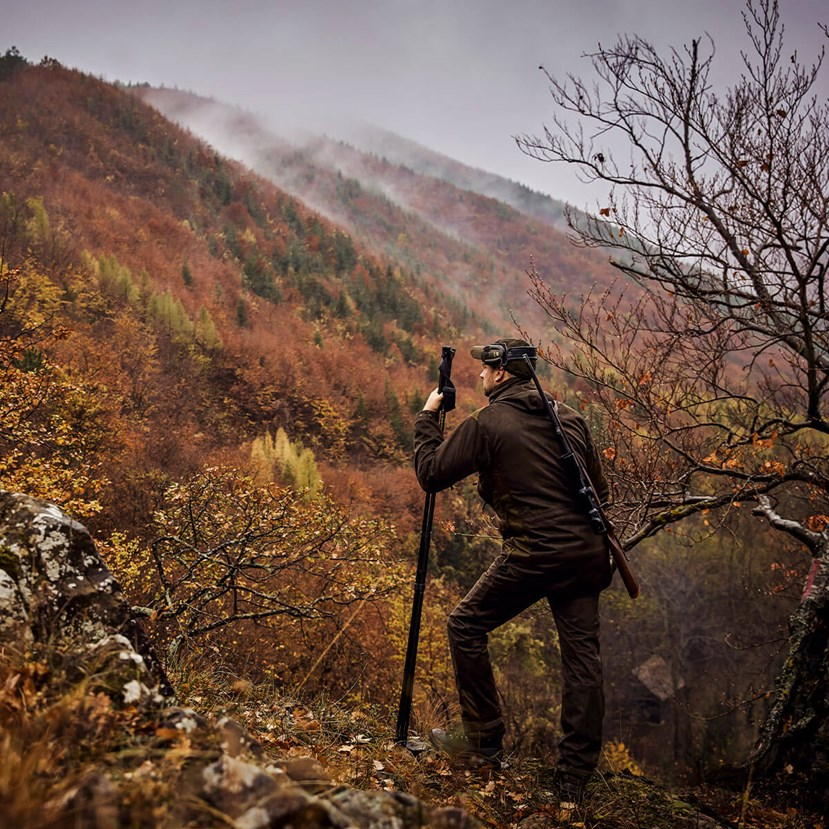
\includegraphics[width=\textwidth,height=0.85\textheight,keepaspectratio]
                {Billeder/Jagtformer/pursch}
            % Alternativt brug en af disse stilrene billeder:
            % \includegraphics[width=\textwidth]{highseat-snow-forest-hunter.jpg}
            % \includegraphics[width=\textwidth]{hunter-leaning-tree-rifle.jpg}
        \end{column}
    \end{columns}
    
\end{frame}